\documentclass{amsart}
\usepackage{graphicx}
\usepackage[margin=3cm]{geometry}
\usepackage{multicol}
\usepackage{amsmath}
\usepackage{caption}
\usepackage{mathrsfs}
\usepackage{float}
\usepackage{xcolor}
\usepackage{subfigure}
% Para tablas:
\usepackage{booktabs}
\usepackage{multirow}
% Para hipervínculos:
\usepackage{hyperref}
\hypersetup{
    colorlinks=true,
    linkcolor=magenta,
    filecolor=magenta,      
    urlcolor=black,
    pdftitle={Reforestation Logistic Transport Optimization},
    pdfpagemode=FullScreen,
    citecolor = blue
    }
\urlstyle{same}
\usepackage[english]{babel}
\usepackage[babel]{csquotes}
\usepackage[backend=biber, style=apa]{biblatex}
\DeclareLanguageMapping{english}{english-apa}
\bibliography{Sources/referencias.bib}

\newenvironment{Figura}
{\par\medskip\noindent\minipage{\linewidth}}
{\endminipage\par\medskip}

\begin{document}

% ------------------------------- PORTADA -----------------------------
    \begin{center}
        {\bfseries\LARGE Instituto Tecnológico de Monterrey\par}
        %\vspace{0.5cm}
        {\scshape\Large Escuela de Ingeniería y Ciencias\par}
        \vspace{0.5cm}
        %{\scshape\Huge Reforestation Logistic Transport Optimization\par}
        {\scshape\Huge Roads to Reforestation: Transport Routing Optimization for Reforestation\par}
        \vspace{0.5cm}
        {\small Juan José H. Beltrán | Kevin Martínez-Trinidad | Jesús Ramirez Mendieta | Ricardo Kaleb Flores Alfonso\par}
        %\begin{table}[h]
        %    \begin{tabular}{cccc}
        %    \begin{tabular}[c]{@{}c@{}}Juan José H. Beltrán\\ a00836747@tec.mx\end{tabular} &
        %        \begin{tabular}[c]{@{}c@{}}Kevin Martínez-Trinidad\\ a@tec.mx\end{tabular} &
        %        \begin{tabular}[c]{@{}c@{}}Kaleb Flores-Alfonso\\ a@tec.mx\end{tabular} &
        %        \begin{tabular}[c]{@{}c@{}}Jesús Ramírez-Mendieta\\ a@tec.mx\end{tabular}
        %    \end{tabular}
        %\end{table}
        \vspace{0.3cm}
        {\small \today}
        \vspace{0.5cm}
        
        \rule{15.5cm}{0.1pt}
    \end{center}


% -----------------------------Abstract---------------------------------

\section*{Abstract}
    This paper addresses the optimization of transport logistics in reforestation projects, focusing on minimizing time, hence, costs associated with the delivery of plants to reforestation sites. Using a Vehicle Routing Problem (VRP) framework, we applied mixed-integer linear programming to identify the optimal routes for delivery trucks, considering vehicle capacities and delivery demands. Also, a heuristic solution was implemented, reducing computational time while maintainin near-optimal results. The solution, based on data from the National Forestry Commision in Mexico, shows that the heuristic model offers and efficient approach to managing reforestation logistics.
    
{\small \subsection*{Keywords} Optimization, vehicle routing problem, linear programming, heuristics, logistics, reforestation.}


% -----------------------------Introduction---------------------------------

    \section{Introduction}
        Climate change and droughts are becoming sustancial problems, not only for keeping ecosystems in harmony, but also for human activities. Deforestation is one of the main causes of droughts, in addition to accelerating climate change. In Mexico, deforestation is a bigger problem than is believed, as it is often carried out illegally or irresponsibly. Meanwhile, reforestation programs allow to reduce the negative effects of deforestation, oganizations like CONAFOR (National Forestry Commission, in Mexico) receive a limited amount of resources and have a maximum period of a few months a year to carry out this kind of project.

         Consequently, a model that indicates which are the optimal routes and the appropriate time to carry them out, thus reducing the time and economic expense of the activity, is necessary to increase as much as possible the probabilities of successfully completing the project, using the least amount of resources possible.
         
         The Vehicle Routing Problem (VRP) is one of the most studied combinatorial optimization problems in recent decades, mainly due to its relevance for the industry. This consists of determining a set of routes for a fleet of vehicles departing from one or more depots to satisfy the demand of geographically dispersed customers \parencite{Sarmiento2014}.
         
         Studies of VRP applied in logistics can be found in the literature \parencite{Nurprihatin2021}, explores different methods for a rice distribution problem, as Monte Carlo simulations and genetic algorithm, staying with a two-steps linear programming method, a transportation model followed by a Capacitated Vehicle Routing Problem. The study considers other transportation methods like ships and planes and designs a conditional methodology combining the steps mentioned before. Meanwhile, Khan \parencite{Khan2014} models a mosquito coil distribution as an assignment problem, considering multiple clients and 3 warehouses. In Feillet \parencite{Feillet2014}, a multiday VRP based on time-classes is introduced to address a problem of transportation of people with dissabilities, where each customer is served almost daily with some consistency being expected in the service, the solution is found using a large neighborhood search heuristic, with each iteration solving a complex VRP with multiple time windows and no waiting time.
         

        \subsection{Objective}        
        The objective of this paper is to minimize both distance and consequently, time, consumed by the trucks that transport the plants to the planting site. To do this, it is proposed to build a work plan that contains ordered routes that allow CONAFOR to make all deliveries in the shortest time possible.
        



% -----------------------------Methodology---------------------------------

\section{Methodology}
    \subsection{Problem Definition}
    Is the intention, through a mathematical model and/or a heuristic algorithm, to provide the staff of Comisión Nacional Forestal (CONAFOR) a method to optimally plan the routes necessary to comply the number of individuals (see Table \ref{tab:especies}) that will be necessary for each section of the reforestation land (Figure \ref{fig:tablaDePoligonos}). 

    After a brief analysis, it can be observed that the project has many similarities with VRP (Vehicule Routing Problem) models, specifically VRP with split deliveries. These problems are characterized by having a source node (depot), which supplies resources to all other nodes, which can be satisfied in several deliveries. From the source node, k vehicles depart, which can have identical or different load capacities \parencite{Dror}.
    
    For this model, given the limited information on the paths available, it was decided to implement the Euclidean distance as the cost of taking each edge. On the other hand, since the number of vehicles available is not known, it was decided to set the number of vehicles as the minimum number of cycles needed to meet all the demands, defining a cycle as one that starts leaving the origin node and ends arriving at the same node. 

    To obtain the distances between the nodes, the image with the geographic location of the polygons provided by CONAFOR (Figure \ref{fig:tablaDePoligonos}) was used, considering the scale in meters presented. A Python code was implemented allowing to obtain the distance between each node by simply entering the approximate coordinate of the centroid of each one.
        
        \begin{figure}[ht]
            \centering
            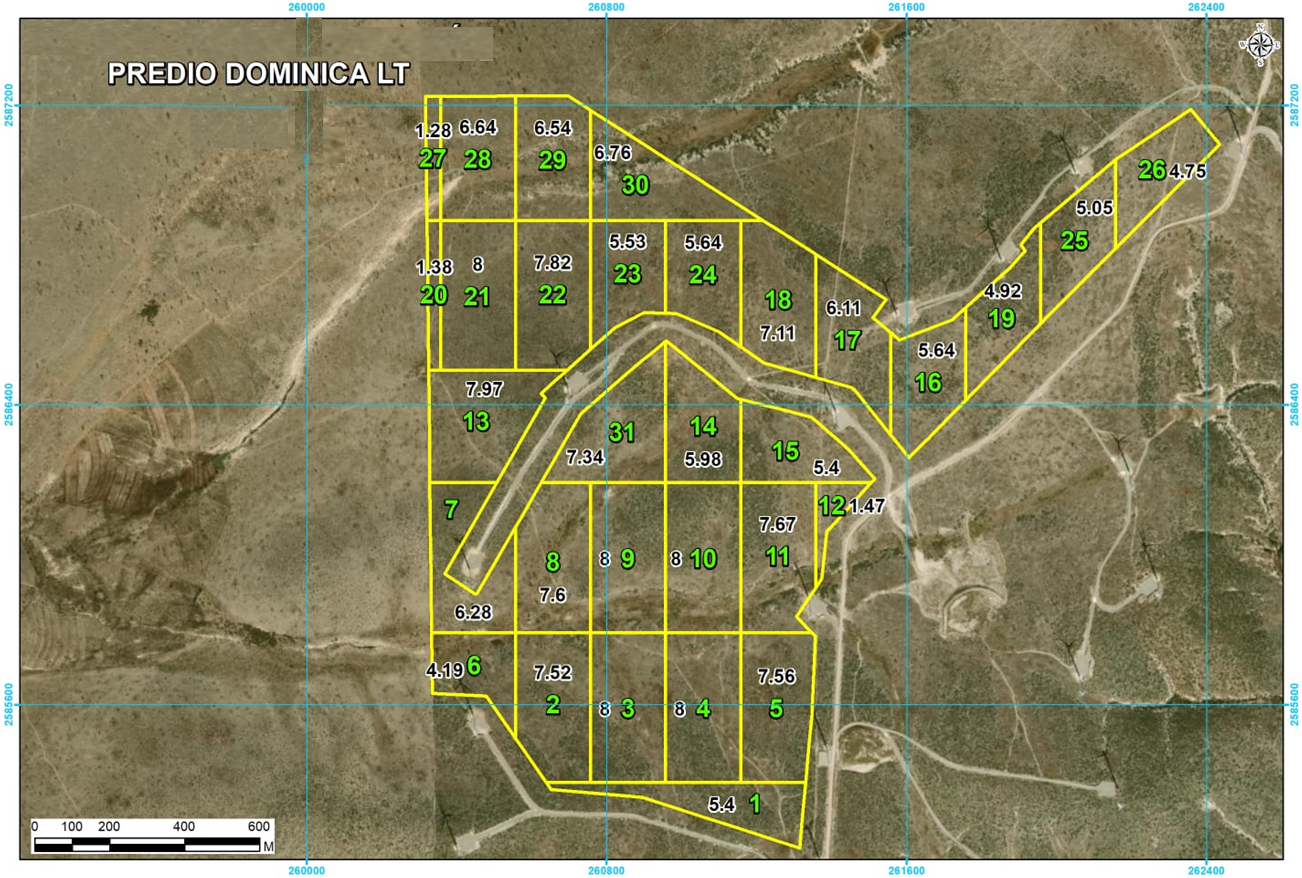
\includegraphics[width=0.5\linewidth]{Sources/Poligonos.png}
            \caption{Sections of land to be reforested. Its numbering and area in hectares are shown.}
            \label{fig:tablaDePoligonos}
        \end{figure}
    
    \subsection{Parameters Considered}
    
    The following values for the parameters were obtained from INECOL.
    
    \begin{itemize}
        \item \textit{Average speed of vehicles:} 20 km/h. Being heavy-duty trucks, these tend to have low acceleration and speed, mainly when dealing with unpaved roads, as in this case study, since there are no established roads on most of the routes and the reforestation area has a uniform altitude.
        \item \textit{Vehicle capacity:} 1 hectare. All vehicles are considered to have identical capacity, as we are actually considering a single vehicle that makes the routes consecutively. According to INECOL, a vehicle loaded to its maximum capacity distributes enough plants to reforest exactly one full hectare.
        \item \textit{Node demands:} The demand corresponds to the area in hectares of each polygon to reforest.
        \item \textit{Loading and unloading time:} 1/2 hour per hectare of load.
        \item \textit{Distance between nodes:} The distances between each pair of nodes are assumed to correspond to the Euclidean distance between the centroids of the polygons they represent in reality.
        \item \textit{Length of a working day:} 8 hours. The standard in Mexico.
    \end{itemize}
    
    %Since the aim is to optimize the time it takes for the vehicles to supply the requested demands, it is necessary to consider the speed at which these vehicles move. Being heavy-duty trucks, these tend to have low acceleration and speed, mainly when dealing with unpaved roads, as in this case study. We consider an average speed of 20 km/h, since there are no established roads on most of the routes and the reforestation area has a uniform altitude.
    
    
    
    \subsection{Problem Simplification}
    
    Note that if it is assumed that all vehicles used have the same capacity (as it happens in this case), many of the nodes need one or more fully loaded trucks to be satisfied, that is, it is necessary to make multiple routes where the vehicles leaves the origin node, arrives at the node to be supplied, unloads all the cargo it carries and returns to the origin node, since it can be proven that these routes are part of the optimal solution. Considering this, most of the delivery cycles can be easily determined just as $\lfloor\frac{\text{\textit{Node demand}}}{\text{\textit{Tuck capacity}}}\rfloor$, leaving only a demand of $\left( \text{\textit{Node demand}} \mod \text{\textit{Truck capacity}} \right)$ to be covered.
    
    For example, in this context, if a node has a demand of 6.28 ha and the vehicles capacity is 1 ha, the model will always carry 6 fully loaded trucks, leaving the node with only the \textit{decimal part} to supply. The order in which these routes are made does not change the cost and calculating the latter does not require great computational capacity.

    It can then be seen that the problem is reduced to determining the routes to follow to supply the \textit{decimal parts} of the demands, thus reducing the complexity of the problem. For this simplified model it can be observed that the number of nodes is reduced to 26, since there are 5 that have integer demands.

    To obtain an optimal solution, a mixed linear programming mathematical model is first proposed (See Section \ref{ModeloMatematico}). This model was executed in the GAMS modeling software and in Python with the help of the PuLP library. However, the proposed model is too complex for the educational license in GAMS, while in Python, the model takes an inadmissible amount of time.

        Because of this, a heuristic solution is proposed (See Section \ref{MetodoHeuristico}), which, through Python code, allows obtaining a very close solution to the optimal one, using much less memory and execution time.

    \subsection{Mathematical Model}\label{ModeloMatematico}
        \subsubsection{Sets} 
        
        
        Set $N=\{1, 2, ... , n\}$ represents the clients (demanding nodes). It is defined $V=N \cup \{0\}$, where $0$ represents the depot. $A$ is the set of arches that join the elements in $V$. $A'$ is the set of arches that join the elements of $N$. With the above, $G=(V, A)$ is a directed and complete graph of nodes $V$ and edges $A$. It's defined $K = \{1, 2, ..., m\}$, representing the vehicles (or the different routes that must be taken).
        

        \subsubsection{Parameters}
        
        
        Let $n \in \mathbb{N}_0$ the number of customers, each with a demand of $q_i : i \in N$. Let $m \in \mathbb{N}$ the maximum number of vehicles (or independent routes) available, all of them with capacity $L \in \mathbb{R}^+$. Note that a lower bound can be placed for $m \geq (\sum q_i) \div Q$. The graph $G$ has costs per unit $c_{a} : a \in A$. Let $\mathcal{M}$ a constant large enough to relate continuous and binary variables in constraints that is at least equal to the maximum demand. Let $v$ a constant corresponding to the average speed of vehicles in meters/hour, and $t$ a constant corresponding to the charging or discharging time measured in hours.


        \subsubsection{Variables}
        
        
        Let $x_{ijk}$ a binary variable that takes value $1$ if vehicle $k$ uses the edge $(i, j)$ on his route, or take value $0$ if it's not used. Similarly, $w_{ijk} \geq 0$ represents the amount of material transported by the vehicle $k$, leaving node $i$ and to deliver to the node $j$. Finally $u_{ik} \in \mathbb{Z}^+$ takes a value corresponding to the order in which the node $i$ is visited by the vehicle $k$.

        
        \vspace{0.4cm} Posed as a linear programming problem, it can be written as follows:
            
            \begin{equation}
                Minimize \hspace{0.5cm} v^{-1} \sum_{i \in V} \sum_{j \in V} \sum_{k \in K} c_{ij} x_{ijk} + 2t \sum_{i \in V} \sum_{j \in V} \sum_{k \in K} w_{ijk} \hspace{0.5cm} : i \neq j
            \end{equation}

        $$Subject\hspace{0.07cm} to \hspace{0.5cm} \sum_{j \in V} x_{ijk} - \sum_{j \in V} x_{jik} = 0 \hspace{0.5cm} : i \neq j \hspace{0.5cm} \forall i \in V, \hspace{0.5cm} k \in K$$

        $$\sum_{j \in N} x_{0jk} = 1 \hspace{0.5cm} \forall k \in K$$

        $$ \sum_{i \in V} \sum_{j \in V} w_{ijk} \leq L \hspace{0.5cm} : i \neq j \hspace{0.5cm} \forall k \in K$$

        $$ \sum_{i \in V} \sum_{k \in K} w_{ijk} \geq q_j \hspace{0.5cm} : i \neq j \hspace{0.5cm} \forall j \in N$$

        $$u_{ik} - u_{jk} + n x_{ijk} \leq n - 1 \hspace{0.5cm} : i \neq j \hspace{0.5cm} \forall i,j \in N, \hspace{0.2cm} k \in K$$

        $$w_{ijk} \leq \mathcal{M} x_{ijk} \hspace{0.5cm} \forall i,j \in V, \hspace{0.2cm} k \in K$$

        $$x_{ijk} \in {1, 2} \hspace{0.5cm} \forall i,j \in V, \hspace{0.2cm} k \in K$$
        
        $$w_{ijk} \geq 0 \hspace{0.5cm} \forall i,j \in V, \hspace{0.2cm} k \in K$$
        
        
\vspace{0.4cm}
        The objective function to be minimized is the sum of the product of the costs per arch and the binary that indicates whether it was used or not, multiplied by the reciprocal of the speed, all of this representing the time invested in traveling distances; plus the sum of all the loads delivered multiplied by $2t$, which is the loading/unloading time, which is assumed to vary linearly depending on the number of plants to be unloaded. 
        
        
        The first group of constraint conserves the flow of vehicles. The second one ensures that all cars pass through node zero (depot). The third constraints group corresponds to the maximum load of each vehicle. The fourth is to satisfy the demands of each customer. The fifth aim to avoid subtours, by assigning each node a positive integer corresponding to the order in which they are visited by each vehicle. Finnaly, the last three group of constraints are about the nature of the variables: $x_{ijk}$ must equal zero only if $w_{ijk}$ is equal to $0$, and must be equal to $1$ otherwise. $x_{ijk}$ is a binary variable. $w_{ijk}$ must be greater than or equal to zero to avoid transporting a negative amount of material (plants).

        \subsection{Heuristic Method}\label{MetodoHeuristico}
        A greedy heuristic algorithm was chosen, which starts by completely supplying the demand of the node furthest from the depot, and then unloads the remaining resource at the node closest to the one previously visited. This makes deliveries more efficient, because having visited and completely supplied the furthest node, no matter where you move, you always get closer to the base. Because the furthest customers are the ones that generate the most costs, this algorithm allows us to reduce the number of times it is necessary to travel to a distant node.
        
        
        \subsection{Model Assumptions and Limitations}
        The assumptions of the model and the limitations they cause in it are stated below, as well as posible solutions for further works.
        
            \subsubsection{Euclidean Distance}
        
            Since the Euclidean distance between nodes is considered, it is ignored that this metric will become misleading once some hectares begin to be reforested, since it will be impossible to cross them on the route. A possible solution would be to consider dynamic distances according to the reforested spaces; or directly consider static distances corresponding to routes that are always guaranteed to be available. In this last case the modification would only be a change of values in the parameters.
            
            \subsubsection{Load Distribution}
            
            The way the load is distributed in the vehicles is not subject to modification, since it is assumed that they are always loaded with the species and specimens necessary to reforest exactly one hectare. Therefore, it cannot be ruled out that there is a better solution by altering this method.
            
        
        \subsection{Ordering the Routes}\label{OrderRoutes}
        Having obtained the optimal routes, it is important to make a visit plan, so the minimum of work days is determined. Assuming that the routes are completely independent of each other and can be reordered at will, the following mathematical model is proposed:
        
        $i$ routes asociated to a $c_i$ cost. We model the problem with binary variables
        $x_{i,t}$, which take the value of 1 if the route $i$ will be done in the day $t$ and binary variables $d_t$, which take the value of 1 if at least one route is programmed to be done in the day $t$.
        Posed as a linear programming problem, it can be written as follows:
        
        \begin{equation}
            Minimize \hspace{0.2cm} \sum^n_{i=1}d_i
        \end{equation}
        $$Subject\hspace{0.07cm} to \hspace{0.5cm} \sum^n_{i=1}c_i*x_{i,t} =l= 8 * d_t$$
        $$\sum^n_{t=1}x_{i,t}=1 \forall i$$
        
        Hence the model is reduced to a problem with two binary variables and less restrictions it can be solved quicker and with less resources.

% -------------------------------------- Results--------------------------------------
    \section{Results}
        \subsection{Solutions with Small Cases}
        In order to compare the results obtained by the mathematical model and the heuristic model with the intention of determine if the closeness of the heuristic solution with the optimal solution is aceptable (less than 5\%), 3 sizes of the problem for which the mathematical model was capable to resolve at razonable times were used, these were tested in 5 samples took randomly: one with 5 nodes (Appendix: Table \ref{tab:5nodos}), another with 10 nodes (Appendix: Table \ref{tab:10nodos}), and one with 12 nodes (Appendix: Table \ref{tab:12nodos}). "P.D.F.O" abbreviates "percentage distance from optimum", considering the general solution: integer part plus decimal part. In order to guarantee the equality of conditions between our samples, no other zero demand nodes besides of the base were included. Likewise, in Table \ref{tab:TiemposDeComputo} is posible to visualize the difference of processing time between the 3 different sizes for the mathematical model, as well as for the heuristic one.
    
            
            \begin{table}[ht]
                \scriptsize
                \begin{tabular}{lrrr}
                \toprule
                \multicolumn{1}{c}{\textbf{\begin{tabular}[c]{@{}c@{}}Problem Size\\ (\# Nodes)\end{tabular}}} &
                  \multicolumn{1}{c}{\textbf{\begin{tabular}[c]{@{}c@{}}Average Computing Time\\ (Mathematical Model)\end{tabular}}} &
                  \multicolumn{1}{c}{\textbf{\begin{tabular}[c]{@{}c@{}}Average Computing Time\\ (Heuristic Model)\end{tabular}}} &
                  \multicolumn{1}{c}{\textbf{\begin{tabular}[c]{@{}c@{}}Average Percentage\\ Distance\end{tabular}}} \\
                  \midrule
                n = 5  & 0.27 s    & 0.0046 s & 1.16\%  \\
                n = 10 & 52.48 s   & 0.0488 s & 0.045\% \\
                n = 12 & 1041.7 s  & 0.0192 s & 0.31\%  \\
                n = 31 & +24 hours & 0.005 s  & — \\ 
                \bottomrule
                \end{tabular}
                \vspace{10pt}
                \caption{Computing times for different problem sizes and different soluton methods.} \label{tab:TiemposDeComputo}
            \end{table}
            
    
            \subsection{Complete Solution}
            
            The optimization problem ended having the next number of sets, variables and parameters:
        \begin{itemize}
            \item A total of 26 nodes (excluding 5 nodes which have an integer demand) and, consequently, 676 arches.
            \item A total 20670 decisión variables, taking in count 3 variables groups: 10140 binary variable $x_{ijk}$, 10140 positive variable $w_{ijk}$, and 390 positive integer variables $u_{ik}$. 
            \item A total of 707 parameters formed by 676 $c_{i,j}$, 26 $q_i$, $m$, $L$, $t$, $M$ and $V$. (See Section \ref{ModeloMatematico} for parameters definitions).
        \end{itemize}
        
            \subsubsection{Exact Solution}
            Given the size of the problem and our computers' capacities, it wasn't possible to solve it with the mathematical model in a reasonable time (less than 48 hours), therefore, we present the colution obtained through the heuristic method.
            
            \subsubsection{Heuristic Solution}
            In total, we obtained 15 different routes needed to satisfy the demand of the decimal part of the nodes, shown in Appendix: Table \ref{tab:ParteDecimal}. Likewise, two of the routes of the proposed model are shown graphically (see Figure \ref{fig:RutasDeEjemplo}). The rest of the routes can be accessed in Appendix.

        \begin{figure}[h!]
            \begin{center}
                \subfigure[Route 1.]{
                    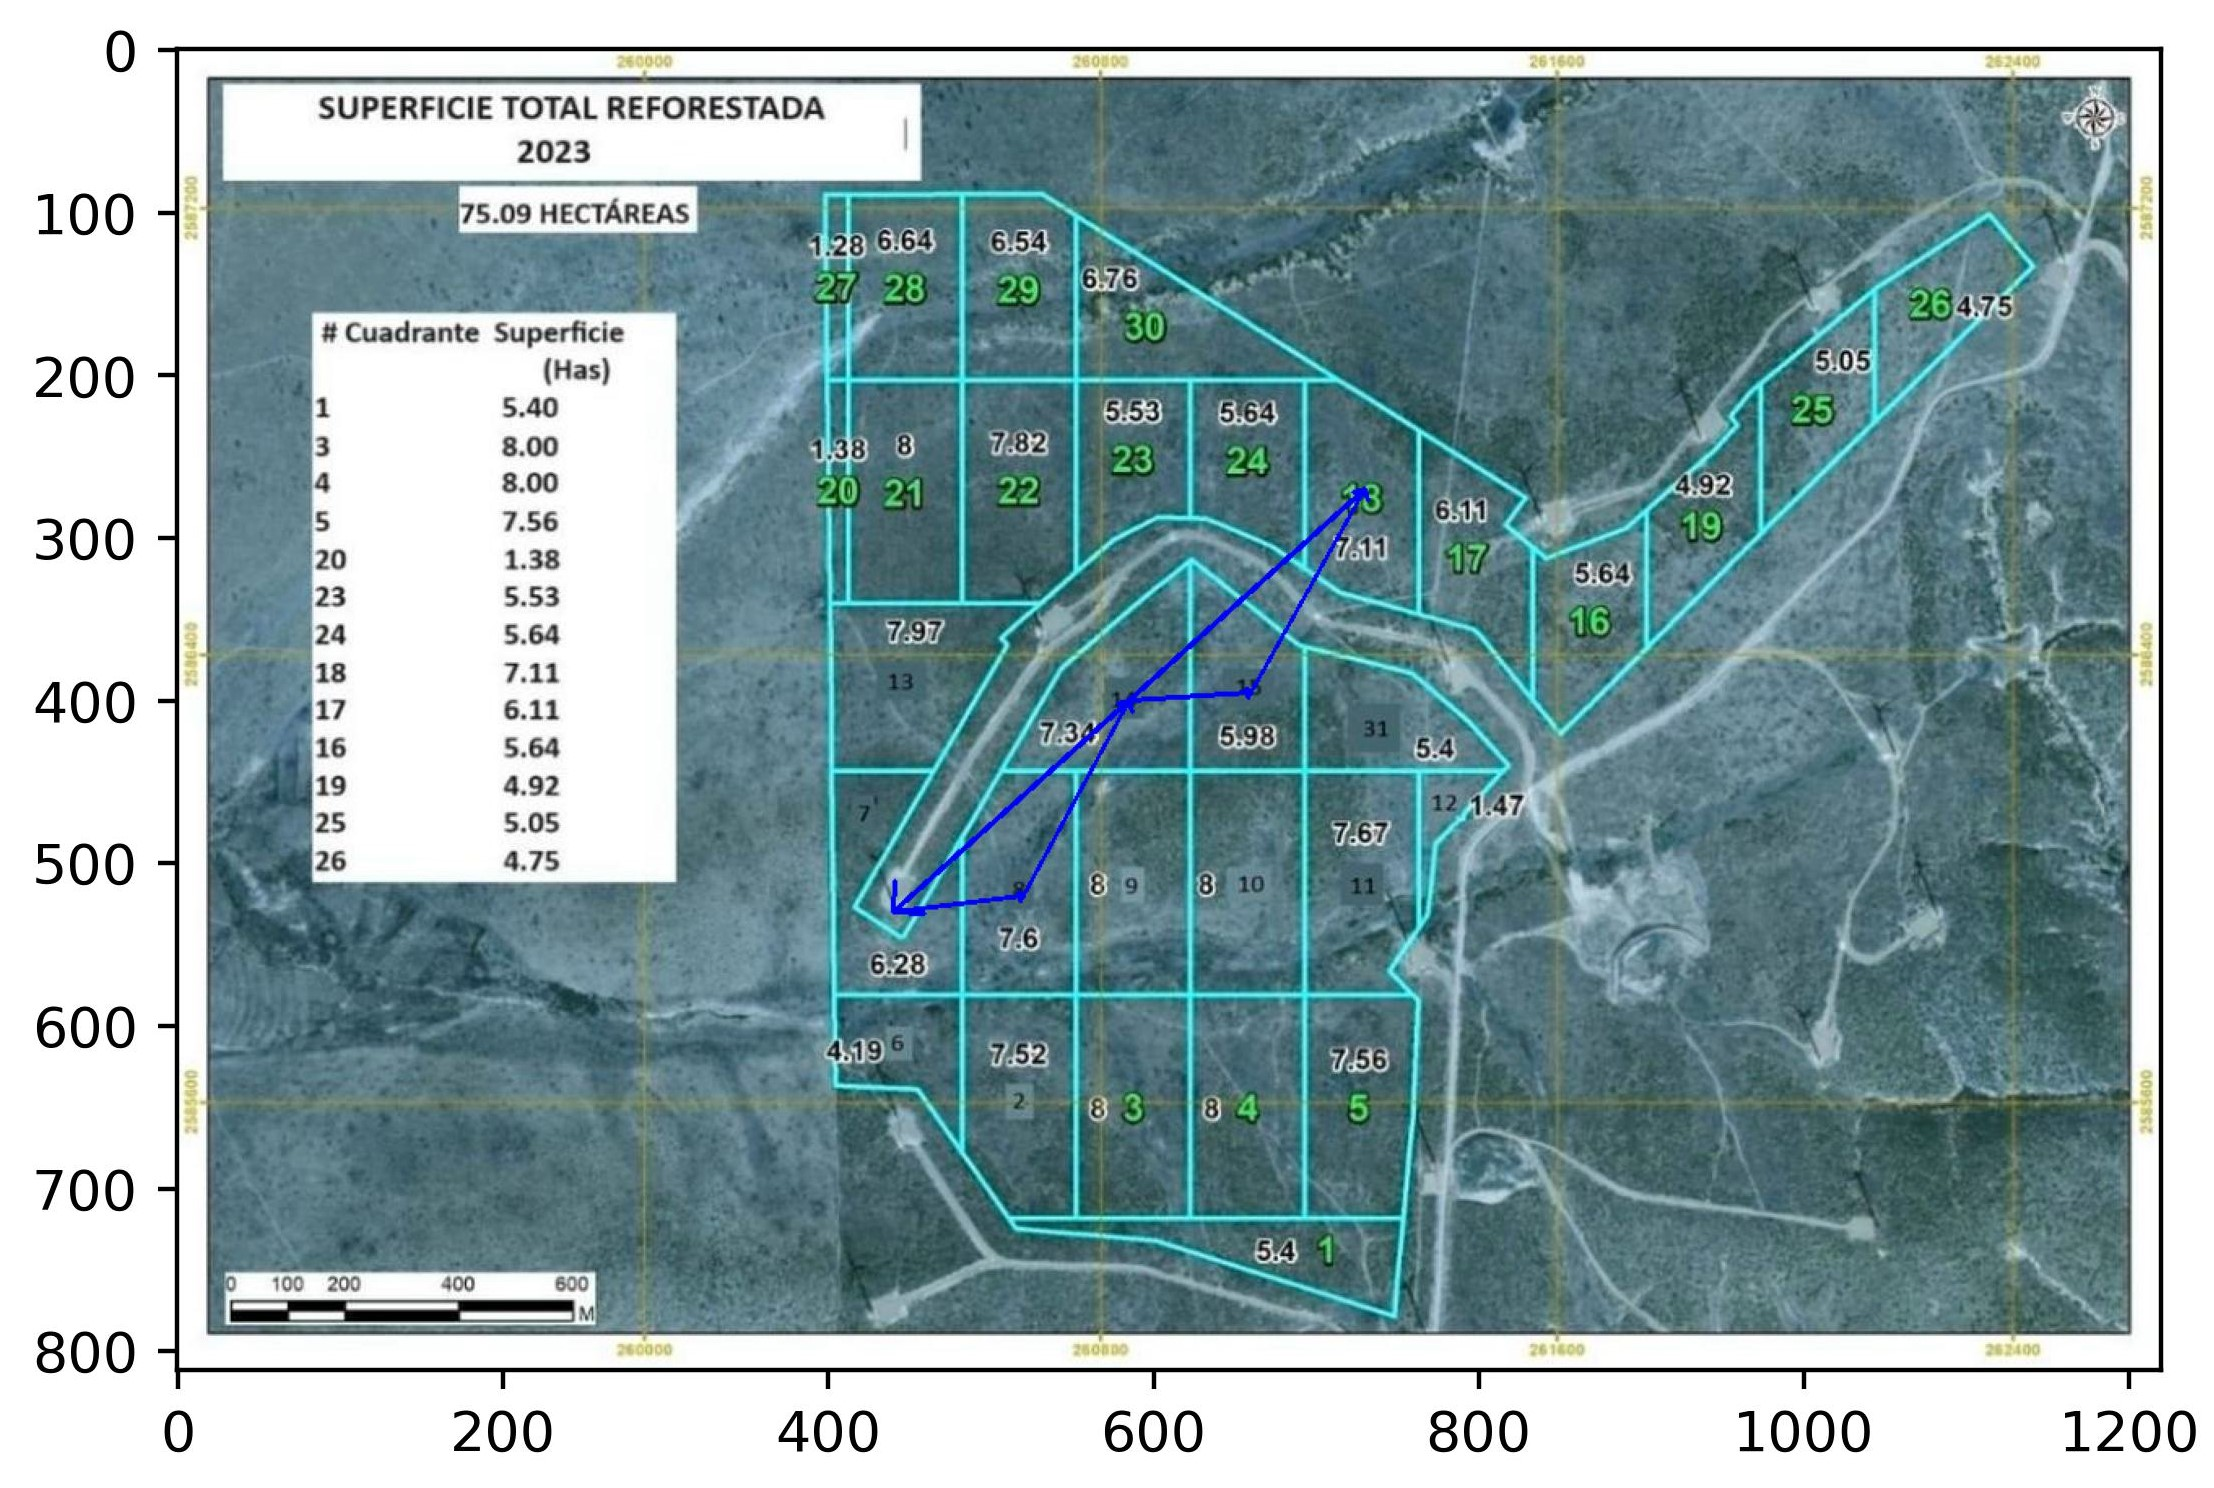
\includegraphics[width=0.48\linewidth]{Sources/Ruta_3.jpg}
                }
                \subfigure[Route 13.]{
                    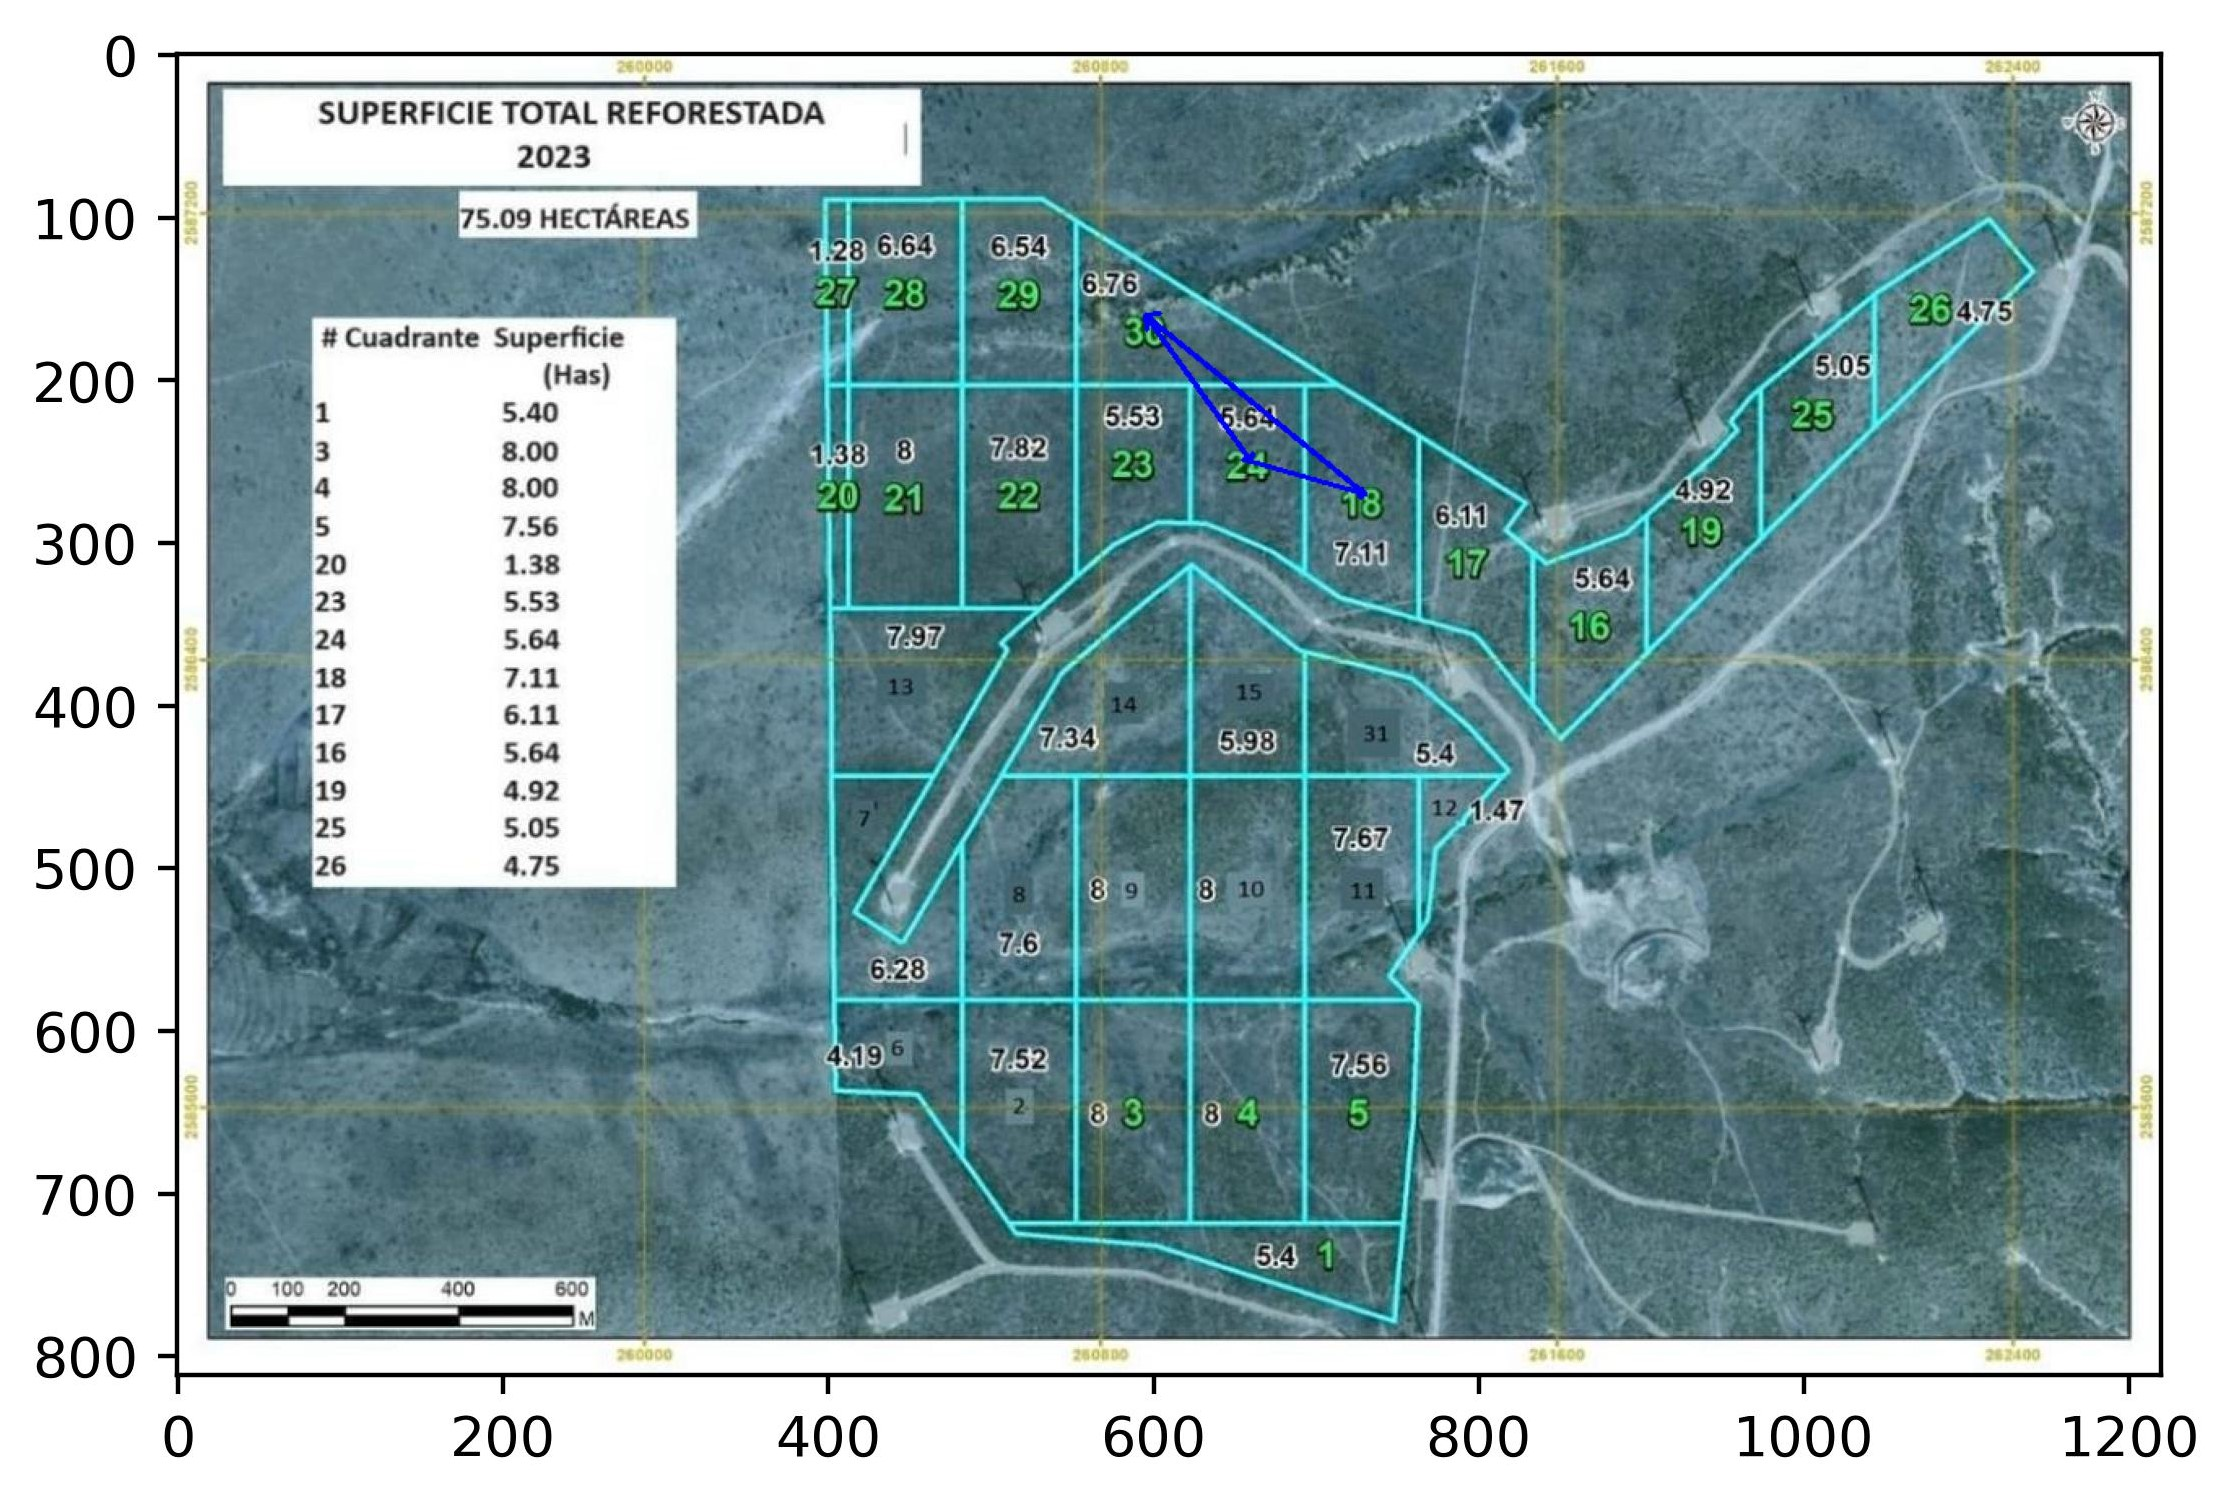
\includegraphics[width=0.48\linewidth]{Sources/Ruta_13.jpg}
                }
                \caption{Some routes that are part of the heuristic solution.}
                \label{fig:RutasDeEjemplo}
            \end{center}
        \end{figure}
            
            For the integer part of the algorithm, 162.68 hours would be needed, while for the decimal part, 15.18 would be needed, hence, the result of the objective function is:
            
            $$z^* = 197.86 \text{ hours}$$

            Equivalent to 25 working days of 8 hours each if we consider only one vehicle, although this time can be improved if several vehicles operate simultaneously. It is important to mention that this solution requieres 183 travels, just the estimated minimum estimated by the lower bound $\lceil \sum_{i} q_i \div L \rceil = 183$, showing its feasibility.
            
            Once the routes are ordered by the mathematical model proposed on Section \ref{OrderRoutes} we got a result for 27 days, but the model got a possible maximum of 26 work days, so we decided to do it by hand, which can be observed in Appendix: Table \ref{tab:DistribucionViajes}.
       
            \subsection{Software and Hardware Specifications}
            
            The experimentation for both the mathematical model and the heuristic model, was implemented on a computer with these characteristics.
    
            \begin{itemize}
                \item \textit{PC model:} Dell G15 5520
                \item \textit{Operative system:} Windows 11.
                \item \textit{Hard disk capacity:} 512GB
                \item \textit{RAM memory:} 16GB.
                \item \textit{Type of Processor:} 12th Gen Intel(R) Core(TM)
                \item \textit{Number of cores:} 7
                \item \textit{Softwares:} For the mathematical model PuLP 2.8.0 in Python with the CPLEX license of IBM was used. For the heuristic model Pandas 2.2 in Python was used.
            \end{itemize}



    
    
% -----------------------------Discussion---------------------------------

    \section{Discussion}
    
    As often happens in this kind of problems, the exact solution resulted to be too much expensive, both in time and memory, therefore, the heuristic model was used at the end.
    
    Moreover, the results obtained by heuristics and the mathematical model for ordering the routes are congruent with the approximate time for the project given by CONAFOR. The organization expects to be able to complete the reforestation in less that a month, while in an ideal scenerario, where no external issue affect the delivery times, the project could be completed in 26 days using the methodology described in this paper, successfully reducing the economic cost and time needed.

    
% -----------------------------Conclusion---------------------------------
    \section{Conclusions}
    Exact solutions based on the mathematical models permits to find the best possible way to solve a problem, which is translated to a considerable reduce of cost. However, there are some cases, like the one presented in this paper, where finding these solutions become inconveniently large in terms of time and memory, at least for most of the commercial computers. This is when hueristics gain relevance, since finding solutions almost as good as the optimal with much less time and memory needed, is definitely an option to take in count for small projects and/or companies that do not count with great computacional resources. 
    Furthermore, there is no doubt that other aspects can be improved in this project, since some factors as the real distance between nodes and other human and ntural inconv
    
    Finally, it is important to mention some of the limitations for this project. 
    \begin{itemize}
        \item The real distance between nodes and the routes the behicules must follow to go from one node to another is not taken in count.
        \item The already established plants are not consider until this point.
        \item The effect the vehicles' weight could have on the established plants and terrain.
        \item the effect of climatic phenomena.
    \end{itemize}


% -------------------------------------- REFERENCES --------------------------------------
    %\vspace{1cm}
    %\newpage
    \section{References}
    \printbibliography[title={References}, heading=none]


% ----------------------------------------APPENDIXES ----------------------------------
    \newpage
    \section{Apendix}
    
        \subsection{Proposed Work Plan}
        Details for each trip are shown in Table \ref{tab:DistribucionViajes}, as well as the specific order in which they should be performed to minimize the number of work days and successfully meet demand.
        
        \begin{table}[!htp]\centering
            \scriptsize
            \begin{tabular}{lrrrrrr}\toprule
            \textbf{Day} &\textbf{Total Hours} &\textbf{Hours per Tour} &\textbf{Distributed load (Ha)} &\textbf{Tour} &\textbf{Iterations} \\\midrule
            1 &1.000 &1.000 & \{0.40, 0.56, 0.04\} &\{1 , 5, 11\} &1 \\
            1 &5.700 &1.140 & \{1\} & \{1\} &5 \\
            2 &7.790 &1.113 &\{1\} & \{5\} &7 \\
            3 &7.800 &1.114 &\{1\} &  \{4\} &7 \\
            4 &1.100 &1.100 &\{1\} &\{4\} &1 \\
            4 &6.670 &1.112 &\{1\} &\{3\} &6 \\
            5 &2.220 &1.110 &\{1\} &\{3\} &2 \\
            5 &5.367 &1.073 &\{1\} &\{10\} &5 \\
            6 &3.220 &1.073 &\{1\} &\{10\} &3 \\
            6 &4.320 &1.080 &\{1\} &\{9\} &4 \\
            7 &4.320 &1.080 &\{1\} &\{9\} &4 \\
            7 &1.000 &1.000 &\{0.19, 0.52, 0.29\} &\{6, 2, 8\} &1 \\
            7 &2.254 &1.127 &\{1\} &\{2\} &2 \\
            8 &5.636 &1.127 &\{1\} &\{2\} &5 \\
            8 &2.186 &1.093 &\{1\} &\{8\} &2 \\
            9 &5.464 &1.093 &\{1\} &\{8\} &5 \\
            9 &2.260 &1.130 &\{1\} &\{6\} &2 \\
            10 &2.260 &1.130 &\{1\} &\{6\} &2 \\
            10 &1.000 &1.000 &\{0.28, 0.31, 0.34, 0.07\} & \{7, 8, 14, 15\} &1 \\
            10 &4.440 &1.110 &\{1\} &\{7\} &4 \\
            11 &2.222 &1.111 &\{1\} &\{7\} &2 \\
            11 &5.267 &1.053 &\{1\} &\{14\} &5 \\
            11 &2.107 &1.053 &\{1\} &\{14\} &2 \\
            12 &1.000 &1.000 &\{0.75, 0.05, 0.2\} &\{26, 25, 19\} &1 \\
            12 &4.436 &1.109 &\{1\} &\{26\} &4 \\
            12 &2.169 &1.084 &\{1\} &\{25\} &2 \\
            13 &3.253 &1.084 &\{1\} &\{25\} &3 \\
            13 &4.250 &1.063 &\{1\} &\{19\} &4 \\
            14 &1.000 &1.000 &\{0.72, 0.28\} &\{19, 16\} &1 \\
            14 &5.230 &1.046 &\{1\} &\{16\} &5 \\
            14 &1.000 &1.000 &\{0.36, 0.11\} &\{16, 17\} &1 \\
            15 &3.060 &1.020 &\{1\} &\{17\} &3 \\
            15 &3.060 &1.020 &\{1\} &\{17\} &3 \\
            15 &1.000 &1.000 &\{0.63, 0.37\} &\{11, 12\} &1 \\
            16 &4.280 &1.070 &\{1\} &\{11\} &4 \\
            16 &3.220 &1.070 &\{1\} &\{11\} &3 \\
            17 &1.060 &1.060 &\{1\} &\{12\} &1 \\
            17 &1.000 &1.000 &\{0.10, 0.4, 0.5\} &\{12, 31, 15\} &1 \\
            17 &5.215 &1.043 &\{1\} &\{31 &\} \\
            18 &1.000 &1.000 &\{0.28, 0.64, 0.08\} &\{27, 28, 29\} &1 \\
            18 &1.100 &1.100 &\{1\} &\{27\} &1 \\
            18 &5.450 &1.090 &\{1\} &\{28\} &5 \\
            19 &1.090 &1.090 &\{1\} &\{28\} &1 \\
            19 &6.400 &1.067 &\{1\} &\{29\} &6 \\
            20 &1.000 &1.000 &\{0.46,0.54\} &\{29,30 &1\} \\
            20 &6.290 &1.048 &\{1\} &30 &6 \\
            21 &1.000 &1.000 &\{0.22, 0.34\} &\{30, 24\} &1 \\
            21 &5.104 &1.021 &\{1\} &\{24\} &5 \\
            21 &1.000 &1.000 &\{0.17, 0.53, 0.3\} &\{22, 23, 24\} &1 \\
            22 &4.163 &1.041 &\{1\} &\{23\} &4 \\
            22 &1.041 &1.041 &\{1\} &\{23\} &1 \\
            22 &1.000 &1.000 &\{0.38, 0.62\} &\{20, 22\} &1 \\
            22 &1.090 &1.090 &\{1\} &\{20\} &1 \\
            23 &5.400 &1.080 &\{1\} &\{21\} &5 \\ 
            23 &2.160 &1.080 &\{1\} &\{21\} &2 \\
            24 &7.400 &1.057 &\{1\} &\{22\} &7 \\
            25 &7.609 &1.087 &\{1\} &\{13\} &7 \\
            26 &1.000 &1.000 &\{0.97, 0.03\} &\{13, 22\} &1 \\
            26 &5.204 &1.041 &\{1\} &\{15\} &5 \\
            26 &1.000 &1.000 &\{0.41\} &\{15\} &1 \\
            \bottomrule
            \end{tabular}
            \vspace{10pt}
            \caption{Complete work plan for one truck.}\label{tab:DistribucionViajes}
        \end{table}
        
        \subsubsection{Results of the Decimal Part}
        Table \ref{tab:ParteDecimal} presents the routes obtained through the heuristic method to optimize time of the decimal part of the problem.
        
        
        \begin{table}[!htp]\centering
        \scriptsize
        \begin{tabular}{lc} \toprule
        \textbf{\#} & \textbf{Route} \\\midrule
        1 & Base → Node 1 → Node 5 → Node 11 → Base \\
        2 & Base → Node 6  → Node 2 → Node 8 → Base \\
        3 & Base → Node 7 → Node 8 → Node 14 → Node 15 → Base \\
        4 & Base → Node 26 → Node 25 → Node 19 → Base \\
        5 & Base → Node 27 → Node 28 → Node 29 → Base \\
        6 & Base → Node 20 → Node 22 → Base \\
        7 & Base → Node 13 → Node 22 → Base \\
        8 & Base → Node 29 → Node 30 → Base \\
        9 & Base → Node 11 → Node 12 → Base \\
        10 & Base → Node 19 → Node 16 → Base \\
        11 & Base → Node 22 → Node 23 → Node 24 → Base \\
        12 & Base → Node 12 → Node 31 → Node 15 → Base \\
        13 & Base → Node 30 → Node 24 → Base \\
        14 & Base → Node 16 → Node 17 → Base \\
        15 & Base → Node 15 → Base \\
        \bottomrule
        \end{tabular}
        \vspace{10pt}
        \caption{Work plan for the decimal part of the demand.}\label{tab:ParteDecimal}
    \end{table}
        
            \subsubsection{Route Images}
            A link to a \href{https://github.com/JuanjoBelt/VRP-ReforestationTransportLogistics/tree/5030293089820a896e177f198d9ab7f23ada59e7/Resources/RouteImages}{\underline{GitHub folder}} with images showing the routes mentioned in our work plan on geographic space is provided for illustrative purposes.
        
        \subsection{Required Distribution of Species per Hectare}
        CONAFOR has established the following planting requirements (Table \ref{tab:especies}), which are identical for each hectare to be reforested. These requirements are scaled, maintaining their proportions between species when dealing with fractions of hectares.
        
        \begin{table}[h!]
            \scriptsize
            \begin{tabular}{llrr}
            \toprule
            \multicolumn{1}{c}{\textbf{No.}} &
              \multicolumn{1}{c}{\textbf{Species}} &
              \multicolumn{1}{c}{\textbf{Percentage of Specimens}} &
              \multicolumn{1}{c}{\textbf{Specimens per Ha.}} \\
              \midrule
            \multicolumn{4}{c}{\textbf{Rosetophilous Crasifolia Species (48.85\%)}}  \\
            \midrule
            1          & Agave lechuguilla               & 6.2977        & 33        \\
            2          & Agave salmiana                  & 29.9618       & 157       \\
            3          & Agave scabra                    & 6.2977        & 33        \\
            4          & Agave Striata                   & 6.2977        & 33        \\
            \midrule
            \multicolumn{4}{c}{\textbf{Crassulaceae Species (33.97\%)}}              \\
            \midrule
            5          & Cylindropuntia imbricata        & 3.8168        & 20        \\
            6          & Opuntia cantabrigiensis         & 4.1985        & 22        \\
            7          & Opuntia engelmannii             & 3.8168        & 20        \\
            8          & Opuntia leucotricha             & 4.9618        & 26        \\
            9          & Opuntia robusta                 & 8.5878        & 45        \\
            10         & Opuntia streptacantha           & 8.5878        & 45        \\
            \midrule
            \multicolumn{4}{c}{\textbf{Woody species (13.16\%)}}                  \\
            \midrule
            11         & Prosopis laevigata              & 13.1679       & 69        \\
            \midrule
            \multicolumn{4}{c}{\textbf{Arborescent Rosetophilous Species (4.01\%)}} \\
            \midrule
            11         & Yucca filifera                  & 4.0076        & 21        \\
            \midrule
            \multicolumn{2}{c}{\textbf{Total}}           & 100           & 524   \\
            \bottomrule
            \end{tabular}
            \vspace{10pt}
            \caption{Distribution of species to be planted.}\label{tab:especies}
        \end{table}
        
        
        
        \subsection{Solutions Obtained from Different Nodes Number}
        Experimental results of the heuristic method are presented against the mathematical model when solving reduced versions of the problem, of different sizes (5 nodes in Table \ref{tab:5nodos}, 10 nodes in Table \ref{tab:10nodos}, and 12 nodes in Table \ref{tab:12nodos}), made up of a random sample of the nodes of the original problem.
        
        \begin{table}[h!]
                \scriptsize
                \begin{tabular}{llrrrrrr}
                \toprule
                \multicolumn{1}{c}{\textbf{\#}} &
                  \multicolumn{1}{c}{\textbf{Sample Nodes}} &
                  \multicolumn{1}{c}{\textbf{\begin{tabular}[c]{@{}c@{}}Optimum\\ (M.M.)\end{tabular}}} &
                  \multicolumn{1}{c}{\textbf{\begin{tabular}[c]{@{}c@{}}Time\\ (M.M.)\end{tabular}}} &
                  \multicolumn{1}{c}{\textbf{\begin{tabular}[c]{@{}c@{}}Solution\\ (H.M.)\end{tabular}}} &
                  \multicolumn{1}{c}{\textbf{\begin{tabular}[c]{@{}c@{}}Time\\ (H.M.)\end{tabular}}} &
                  \multicolumn{1}{c}{\textbf{\begin{tabular}[c]{@{}c@{}}Integer\\ Part\end{tabular}}} &
                  \multicolumn{1}{c}{\textbf{P.D.F.O.}} \\
                \midrule
                1 & \{1, 18, 20, 23, 26\} & 2.33 & 0.05 s & 2.483 & 0.004 s & 16.433 & 0.81\% \\
                2 & \{1, 7, 11, 18, 20\}  & 1.97 & 0.05 s & 2.112 & 0.007 s & 21.245 & 0.61\% \\
                3 & \{1, 2, 8, 16, 18\}   & 2.40 & 0.6 s  & 2.547 & 0.003 s & 26.481 & 0.50\% \\
                4 & \{5, 17, 18, 19, 29\} & 2.33 & 0.1 s  & 2.352 & 0.003 s & 24.83  & 0.08\% \\
                5 & \{6, 7, 13, 18, 30\}  & 1.41 & 0.1 s  & 2.414 & 0.006 s & 25.094 & 3.78\% \\
                \bottomrule
                \end{tabular}
                \vspace{10pt}
                \caption{Contrast between the solutions and computation times of the mathematical model and the heuristic method in 5-node test cases.} \label{tab:5nodos}
            \end{table}
            
            

            \begin{table}[h!]
                \scriptsize
                \begin{tabular}{llrrrrrr}
                \toprule
                \multicolumn{1}{c}{\textbf{\#}} &
                  \multicolumn{1}{c}{\textbf{Sample Nodes}} &
                  \multicolumn{1}{c}{\textbf{\begin{tabular}[c]{@{}c@{}}Optimum\\ (M.M.)\end{tabular}}} &
                  \multicolumn{1}{c}{\textbf{\begin{tabular}[c]{@{}c@{}}Time\\ (M.M.)\end{tabular}}} &
                  \multicolumn{1}{c}{\textbf{\begin{tabular}[c]{@{}c@{}}Solution\\ (H.M.)\end{tabular}}} &
                  \multicolumn{1}{c}{\textbf{\begin{tabular}[c]{@{}c@{}}Time\\ (H.M.)\end{tabular}}} &
                  \multicolumn{1}{c}{\textbf{\begin{tabular}[c]{@{}c@{}}Integer\\ Part\end{tabular}}} &
                  \multicolumn{1}{c}{\textbf{P.D.F.O.}} \\
                \midrule
                1 & \begin{tabular}[c]{@{}l@{}}\{2, 8, 13, 16, 17, 18, 20, 22, 28, 29\}\end{tabular} & 5.67 & 233 s & 5.73  & 0.032 s & 56.021 & 0.09\% \\
                2 & \begin{tabular}[c]{@{}l@{}}\{5, 8, 12, 16, 18, 19, 20, 22, 28, 29\}\end{tabular} & 6.00 & 15 s  & 6.049 & 0.005 s & 47.488 & 0.09\% \\
                3 & \begin{tabular}[c]{@{}l@{}}\{2, 5, 6, 7, 11, 17, 18, 20, 22, 30\}\end{tabular}   & 4.69 & 5.8 s & 4.734 & 0.036 s & 55.326 & 0.07\% \\
                4 & \begin{tabular}[c]{@{}l@{}}\{2, 8, 11, 18, 19, 20, 23, 26, 29, 30\}\end{tabular} & 6.14 & 3.9 s & 6.203 & 0.031 s & 50.758 & 0.11\% \\
                5 & \begin{tabular}[c]{@{}l@{}}\{2, 7, 11, 18, 19, 20, 23, 26, 29, 30\}\end{tabular} & 5.81 & 4.7 s & 5.864 & 0.012 s & 49.773 & 0.09\% \\ 
                \bottomrule
                \end{tabular}
                \vspace{10pt}
                \caption{Contrast between the solutions and computation times of the mathematical model and the heuristic method in 10-node test cases.} \label{tab:10nodos}
            \end{table}
            
            
            \begin{table}[h!]
                \scriptsize
                \begin{tabular}{llrrrrrr}
                \toprule
                \multicolumn{1}{c}{\textbf{\#}} &
                  \multicolumn{1}{c}{\textbf{Sample Nodes}} &
                  \multicolumn{1}{c}{\textbf{\begin{tabular}[c]{@{}c@{}}Optimum\\ (M.M.)\end{tabular}}} &
                  \multicolumn{1}{c}{\textbf{\begin{tabular}[c]{@{}c@{}}Time\\ (M.M.)\end{tabular}}} &
                  \multicolumn{1}{c}{\textbf{\begin{tabular}[c]{@{}c@{}}Solution\\ (H.M.)\end{tabular}}} &
                  \multicolumn{1}{c}{\textbf{\begin{tabular}[c]{@{}c@{}}Time\\ (H.M.)\end{tabular}}} &
                  \multicolumn{1}{c}{\textbf{\begin{tabular}[c]{@{}c@{}}Integer\\ Part\end{tabular}}} &
                  \multicolumn{1}{c}{\textbf{P.D.F.O.}} \\
                \midrule
                1 & \{1, 2, 6, 8, 11, 15, 18, 19, 20, 22, 23, 29\} & 7.07 & 63 s & 7.237 & 0.027 s & 62.879 & 0.23\% \\
                2 & \{1, 2, 5, 6, 8, 15, 18, 20, 22, 25, 27, 30\}  & 6.07 & 425 s & 6.763 & 0.010 s & 60.104 & 1.04\% \\
                3 & \{1, 5, 6, 7, 8, 11, 14, 17, 18, 19, 22, 29\}   & 6.04 & 1035 s  & 6.135 & 0.036 s & 71.469 & 0.11\% \\
                4 & \{2, 3, 7, 9, 11, 13, 18, 22, 25, 29, 30\} & 6.01 & 26 s  & 6.107 & 0.010 s & 72.448  & 0.12\% \\
                5 & \{2, 5, 6, 7, 11, 14, 15, 18, 24, 29, 30\}  & 6.54 & 3684 s  & 6.591 & 0.013 s & 72.448 & 0.06\% \\
                \bottomrule
                \end{tabular}
                \vspace{10pt}
                \caption{Contrast between the solutions and computation times of the mathematical model and the heuristic method in 12-node test cases.} \label{tab:12nodos}
            \end{table}
        
        

        \subsection{Implementation of Solution Methods}
        Attached is a link to a \underline{\href{https://github.com/JuanjoBelt/VRP-ReforestationTransportLogistics}{GitHub repository}} containing all the implementations of the solution methods mentioned in this article, as well as all the information necessary to study and replicate it.
        

    
 \end{document}
